%% AgentProp-Bench — arXiv preprint version
%% Compile: pdflatex, bibtex, pdflatex, pdflatex

\documentclass[11pt]{article}

%% === Page layout ===
\usepackage[margin=1in]{geometry}

%% === Math ===
\usepackage{amsmath,amssymb,amsfonts}

%% === Tables ===
\usepackage{booktabs}
\usepackage{multirow}
\usepackage{array}
\usepackage{tabularx}

%% === Graphics ===
\usepackage{graphicx}

%% === Typography ===
\usepackage{microtype}
\usepackage{xspace}
\usepackage{xcolor}

%% === Links ===
\usepackage{hyperref}
\usepackage{url}
\hypersetup{colorlinks=true, citecolor=blue, linkcolor=blue, urlcolor=blue}

%% === References ===
\usepackage[round,authoryear]{natbib}

%% === Authors ===
\usepackage{authblk}

%% === Section formatting ===
\usepackage{titlesec}

%% === Semantic macros ===
\newcommand{\bench}{\textsc{AgentProp-Bench}\xspace}
\newcommand{\eps}{\mathrm{EPS}}
\renewcommand{\Pr}{\mathbb{P}}
\newcommand{\E}{\mathbb{E}}
\newcommand{\ind}{\mathbf{1}}
\newcommand{\interceptor}{\textsc{Interceptor}\xspace}

% ============================================================================
\title{Evaluating Tool-Using Language Agents: Judge Reliability,\\
Propagation Cascades, and Runtime Mitigation in \bench{}}

\author[1]{Bhaskar Gurram\thanks{Corresponding author. Email: gurrambhaskar.ai@gmail.com}}
\affil[1]{Zasti Inc., Ashburn, VA, USA}

\date{}

% ============================================================================
\begin{document}
\maketitle

% === Abstract ===
\begin{abstract}
Automated evaluation of tool-using large language model (LLM) agents is
widely assumed to be reliable, but this assumption has rarely been
validated against human annotation.
We introduce \bench{}, a 2{,}000-task benchmark with 2{,}300 traces
across four domains, nine production LLMs, and a 100-label
human-validated subset.
We quantify judge reliability, characterize error propagation, and
evaluate a runtime mitigation.
Substring-based judging agrees with human annotation at $\kappa{=}0.049$
(chance-level); a three-LLM ensemble reaches $\kappa{=}0.432$ (moderate)
with a conservative bias.
Under validated evaluation, a parameter-level injection propagates to a
wrong final answer with human-calibrated probability ${\approx}\,0.62$
(range 0.46--0.73 across models).
Rejection (catching bad parameters) and recovery (correcting after
acceptance) are independent model capabilities
(Spearman $\rho{=}0.126$, $p{=}0.747$).
A tuned runtime interceptor reduces hallucination on GPT-4o-mini by
23.0 percentage points under a concurrent $n{=}600$ control, but shows
no significant effect on Gemini-2.0-Flash, whose aggressive parameter
rejection eliminates the target failure mode.
All code, data, traces, and human labels are released at
\url{https://github.com/bhaskargurram-ai/agenthallu-bench}.\footnote{Repository
previously published as AgentHallu-Bench; renamed to \bench{} to
reflect the focus on propagation measurement and to avoid confusion
with the concurrently published ``AgentHallu'' paper
\citep{liu2026agenthallu}, which pursues step-level attribution on a
different dataset.}
\end{abstract}

\noindent\textbf{Keywords:}
large language model agents, tool-use hallucination,
error propagation, benchmark, LLM-as-judge,
runtime monitoring, evaluation methodology

\vspace{1em}

% ============================================================================
\section{Introduction}
\label{sec:intro}

Tool-using large language model (LLM) agents translate natural-language
queries into structured API calls, execute those calls, and synthesize
the results into a final answer.
When such an agent hallucinates, the failure is not confined to the
surface token distribution: a mistyped parameter, an ignored tool error,
or an overconfident summary can each corrupt the output.
Agent benchmarks such as $\tau$-bench \citep{yao2024tau},
AgentBench \citep{liu2024agentbench}, and BFCL \citep{yan2025bfcl}
report a single end-to-end correctness number and cannot localize
\emph{where} a failure occurs or \emph{how} it propagates through the
pipeline.

A less visible but equally important gap concerns \emph{how correctness
is measured}.
Most agent benchmarks rely on substring or keyword-match heuristics to
judge whether an agent's final answer matches a reference.
This practice has been questioned in the information retrieval (IR)
community, where studies show that LLM judges and heuristic judges can
disagree substantially on relevance assessments
\citep{soboroff2024dont,thomas2024searcher,alaofi2024fooled}.
If the evaluation itself is unreliable, then every downstream claim about
model ranking, error propagation, or mitigation effectiveness is suspect.

We present \bench{}, a benchmark and methodology designed to address
both gaps.
Our contributions are:
\begin{enumerate}
  \item \textbf{Judge-reliability validation.}
    We show that substring-based evaluation of agent outputs agrees with
    human annotation at $\kappa{=}0.049$ (chance-level), while a
    three-LLM ensemble judge reaches $\kappa{=}0.432$ (moderate
    agreement), validated against 100 stratified human labels
    (Section~\ref{sec:judge}).
  \item \textbf{Stage-level propagation measurement.}
    Under validated evaluation, we define three independent stage
    indicators and show that a parameter-level injection propagates to a
    wrong answer with human-calibrated probability ${\approx}\,0.62$
    (range 0.46--0.73 per model) (Section~\ref{sec:propagation}).
  \item \textbf{Rejection--recovery decomposition.}
    Rejection rate (catching bad parameters) and recovery rate (producing
    a correct answer despite accepting bad parameters) are statistically
    independent across nine models (Spearman $\rho{=}0.126$,
    $p{=}0.747$), revealing that models vary on two orthogonal axes of
    robustness (Section~\ref{sec:rejrec}).
  \item \textbf{Runtime interceptor under concurrent control.}
    A tuned three-layer \interceptor{} reduces hallucination on
    GPT-4o-mini by 23.0~pp under a concurrent $n{=}600$ no-interceptor
    control ($p < 0.001$), but has no significant effect on
    Gemini-2.0-Flash (Section~\ref{sec:interceptor}).
  \item \textbf{Open benchmark release.}
    All 2{,}000 tasks, 2{,}300 traces, 100 human labels, analysis
    scripts, and agent source code are publicly released.
\end{enumerate}

The remainder of this paper is organized as follows.
Section~\ref{sec:related} reviews related work on agent benchmarks,
LLM-as-judge reliability, and agent hallucination.
Section~\ref{sec:ro} states the research objectives.
Section~\ref{sec:dataset} describes the \bench{} dataset.
Section~\ref{sec:method} presents the methodology.
Section~\ref{sec:results} reports results.
Section~\ref{sec:discussion} discusses theoretical and practical
implications.
Section~\ref{sec:limits} acknowledges limitations.
Section~\ref{sec:conclusion} concludes.


% ============================================================================
\section{Related Work}
\label{sec:related}

\subsection{Tool-using LLM agent benchmarks}

The evaluation of tool-using LLM agents has rapidly expanded.
$\tau$-bench \citep{yao2024tau} evaluates agents on multi-step retail
and airline tasks, measuring end-to-end task completion.
\citet{barres2025tau2} extend $\tau$-bench to additional domains.
AgentBench \citep{liu2024agentbench} spans eight environments including
web browsing and database queries.
BFCL \citep{yan2025bfcl} focuses on function-calling accuracy across
multiple programming languages and API styles.
MCPBench \citep{mcpagentbench2026} evaluates agents on real-world API
integration tasks.
Recent surveys \citep{yehudai2025surveyeval,xie2025agentir} provide
comprehensive overviews of agent architectures and evaluation practices.

These benchmarks share a common limitation: they report a single
end-to-end correctness number and do not localize \emph{where} in the
agent pipeline a failure originates.
\bench{} addresses this by decomposing evaluation into three
independently measured stages.

\subsection{LLM-as-judge reliability}

Using LLMs as judges has become widespread in both NLP and IR evaluation.
\citet{zheng2023judging} introduced the LLM-as-judge paradigm with
MT-Bench and Chatbot Arena.
\citet{gu2024surveyjudge} survey the growing LLM-as-judge literature,
identifying position bias, verbosity bias, and self-enhancement bias.
\citet{bavaresco2024llmsjudges} provide a multidimensional analysis of
when LLM judges agree with humans.

In the IR community, judge reliability has received particular scrutiny.
\citet{soboroff2024dont} argue that LLM judges should not replace human
assessors without validation.
\citet{thomas2024searcher} show that LLM judges and human searchers
diverge on relevance criteria.
\citet{alaofi2024fooled} demonstrate that LLM judges can be fooled by
surface-level text manipulation.
\citet{thakur2025judging} benchmark judge reliability across retrieval
tasks.
\citet{fu2025multilingual} extend judge evaluation to multilingual
settings.
\citet{schroeder2024trust} quantify when and why practitioners should
trust LLM-based evaluation.

Our work contributes to this literature by validating an LLM-ensemble
judge against 100 human labels in the specific context of tool-using
agent evaluation, where output format variability (structured data,
error messages, multi-step reasoning) makes heuristic evaluation
particularly unreliable.

\subsection{Hallucination in LLM agents}

Hallucination in standalone LLMs has been extensively surveyed
\citep{huang2024hallucination,lin2025agenthallusurvey}.
Agent-specific hallucination introduces additional failure modes:
parameter fabrication, tool-output misinterpretation, and cross-turn
memory corruption \citep{zhang2025memory}.

Most closely related to our work, \citet{liu2026agenthallu} introduce
AgentHallu, a benchmark for automated hallucination attribution in
LLM-based agents.
AgentHallu performs step-level attribution on 693 trajectories across
five domains, categorizing hallucinations by stage of origin.
\bench{} differs in three respects:
(1)~we use \emph{controlled injection} rather than naturally occurring
errors, enabling causal measurement of propagation rates;
(2)~we validate our evaluation methodology against 100 human labels
($\kappa{=}0.432$), whereas AgentHallu relies on automated attribution;
(3)~we evaluate a runtime interceptor under a concurrent control,
providing mitigation evidence beyond diagnosis.
The two benchmarks address complementary questions: AgentHallu asks
``where did this hallucination come from?'' while \bench{} asks
``if we inject an error here, with what probability does it propagate
there?''

\subsection{Runtime monitoring and mitigation}

Several approaches have been proposed for runtime hallucination
detection and mitigation.
Self-consistency voting \citep{wang2023selfconsistency} samples multiple
reasoning paths and selects the majority answer.
\citet{manakul2023selfcheckgpt} propose SelfCheckGPT for detecting
hallucinations without external references.
\citet{farquhar2024semantic} use semantic entropy to detect
confabulations in free-form LLM generations.
Guardrails and runtime enforcement frameworks
\citep{wang2026agentspec} provide schema-level validation.

Our \interceptor{} combines schema validation, reasoning-keyword
monitoring, and output-consistency checking in a three-layer architecture.
Unlike self-consistency voting (which requires $k\times$ sampling cost),
the \interceptor{} runs in parallel with a single agent execution at
negligible additional cost.

\subsection{Relevance to IR and IS evaluation}

The evaluation-reliability problem we address has direct implications
for the IR and information science (IS) communities.
LLMs are increasingly used for relevance assessment in IR evaluation
\citep{balog2025rankers}, and the reliability of these
assessments directly affects system rankings.
\citet{salemi2024retrieval} study LLMs as relevance judges in retrieval
settings.
\citet{rahmani2024synthetic} examine synthetic data generation for IR
evaluation.
\citet{zhu2024llmir} survey LLM applications in information science.

Our finding that substring-based evaluation agrees with humans at
$\kappa{=}0.049$ (chance-level) has implications beyond agent
benchmarks.
Substring and keyword-match heuristics are common correctness proxies in
question-answering and retrieval-augmented generation (RAG) evaluation
\citep{es2024ragas,niu2024ragtruth}.
The ensemble-judge methodology we validate here---with explicit
per-rater and human-calibrated agreement reporting---transfers directly
to these settings.

\subsection{Research gap}

Existing work provides either end-to-end benchmarks without stage-level
decomposition, or judge-reliability studies without application to agent
evaluation.
No prior work validates an agent evaluation pipeline end-to-end against
human annotation, measures stage-conditional propagation under validated
judging, and evaluates a mitigation under concurrent control---all in
one study.
\bench{} fills this gap.


% ============================================================================
\section{Research Objectives}
\label{sec:ro}

We formulate three research objectives:

\paragraph{RO1: Judge reliability.}
What is the agreement between heuristic substring matching, a
three-LLM ensemble judge, and human annotation on tool-using agent
outputs?
Prior work shows that heuristic evaluation is unreliable for
paraphrased or verbose outputs \citep{soboroff2024dont}.
We quantify this unreliability in the agent-evaluation context and
validate the ensemble as a better---but imperfect---alternative.

\paragraph{RO2: Error propagation under validated evaluation.}
How does a parameter-level injection propagate through the agent
pipeline when correctness is measured by a validated judge?
Prior work either reports end-to-end correctness or attributes
errors post hoc \citep{liu2026agenthallu}.
We measure stage-conditional propagation rates and decompose model
robustness into independent rejection and recovery capabilities.

\paragraph{RO3: Runtime mitigation under concurrent control.}
Can a lightweight runtime interceptor reduce hallucination under a
properly controlled experiment?
Prior interceptor evaluations \citep{wang2026agentspec} typically
compare against historical baselines.
We evaluate under a concurrent $n{=}600$ no-interceptor control on
the same task pool.


% ============================================================================
\section{Dataset: \bench{}}
\label{sec:dataset}

\subsection{Task design and construction}

Each task in \bench{} is a tuple $(q, D, T_q, a^\star)$ where $q$ is a
natural-language query, $D$ is a domain, $T_q$ is a set of available
tools, and $a^\star$ is a reference answer.
Tasks are classified by difficulty: \emph{easy} (single tool call),
\emph{medium} (two-tool chain), and \emph{hard} (three-tool chain or
branching logic).
Tasks and reference answers were generated synthetically using
domain-specific API simulators, then manually verified for correctness.

\subsection{Domain breakdown}

\bench{} comprises 2{,}000 tasks across four domains plus a held-out
retail domain:
\begin{itemize}
  \item \textbf{Calendar} (667 tasks): event creation, schedule queries,
    conflict detection.
  \item \textbf{Weather} (674 tasks): current conditions, forecasts,
    historical comparisons.
  \item \textbf{Medical} (559 tasks): patient lookup, appointment
    scheduling, condition retrieval.
  \item \textbf{Knowledge} (100 tasks): general question-answering
    (ablation only, no tool injection).
  \item \textbf{Retail} (300 tasks, held-out): product search, detail
    inspection, order placement.
\end{itemize}

Table~\ref{tab:dataset} provides a detailed breakdown by domain and
difficulty.

% Source: data/tasks/full_2000_tasks.json
\begin{table}[t]
\centering
\caption{Dataset composition of \textsc{AgentProp-Bench}. $N = 2{,}000$ core + 300 retail.}
\label{tab:dataset}
\small
\begin{tabular}{l r r r r p{4.5cm}}
\toprule
Domain & Tasks & Easy & Med. & Hard & Example query \\
\midrule
Calendar & 667 & 192 & 282 & 193 & Create a meeting on 2024-07-08 at 10:00 for 30 min \\
Weather & 674 & 215 & 248 & 211 & What is the weather in Dubai on 2024-10-12? \\
Medical & 559 & 106 & 237 & 216 & Schedule a checkup for patient P003 \\
Knowledge & 100 & 0 & 46 & 54 & What nationality is the CEO of Samsung? \\
\midrule
Retail (held-out) & 300 & --- & --- & --- & Search catalog for wireless headphones \\
\bottomrule
\end{tabular}
\end{table}


\subsection{Tool schema and simulated environment}

Each domain provides 3--5 tools implemented as deterministic Python
functions with JSON schemas.
Tools validate input parameters against their schemas and return
structured JSON responses.
Invalid parameters produce explicit error messages rather than silent
failures.
This design ensures that parameter-level injection effects are
observable in tool responses.

\subsection{Error-injection protocol}

We use the P2 \emph{semantic-wrong} injection protocol: before the
agent's first tool call executes, we replace a semantically critical
parameter with an incorrect but schema-valid value.
For example, in a weather query for ``London,'' we might replace the
city parameter with ``Manchester''---a valid city but the wrong one.
The injection is applied at the \texttt{parameter\_generation} stage
of the pipeline.

\subsection{Trace collection}

We collected 2{,}300 traces across nine production LLMs:
GPT-4o, GPT-4o-mini, GPT-4.1-mini, GPT-4.1-nano, GPT-3.5-turbo,
o3-mini (OpenAI); Gemini-2.0-Flash, Gemini-2.5-Flash (Google); and
DeepSeek-V3 (via OpenRouter).
For the P2 semantic-wrong condition, we evaluated 200 unique tasks
per model for the six main models (800 rows across four error types)
and 50 tasks for three frontier models (200 rows each).
All models were accessed via their official APIs with default
parameters (temperature 0).

\subsection{Human label collection}

To validate the ensemble judge, we collected 100 human labels on a
stratified sample of P2 semantic-wrong traces.
The sample was stratified across all nine models (10--12 per model)
and three domains (calendar, medical, weather).
One annotator (the first author) labeled each trace as ``correct''
(YES) or ``incorrect'' (NO) by comparing the agent's final answer to
the reference answer.
The labeling criterion matched the ensemble judge prompt: accept minor
wording differences and extra explanation as long as the core fact is
correct.
A second annotator (acknowledged) independently labeled 7 overlapping
traces; inter-annotator agreement on this small overlap was 6/7.

\subsection{Data availability}

All data are publicly available at
\url{https://github.com/bhaskargurram-ai/agenthallu-bench}.
The repository includes task specifications, all result CSVs, analysis
scripts, agent source code, and human annotation labels.
Every numerical claim in this paper traces to a specific file via
inline comments in the \LaTeX{} source.


% ============================================================================
\section{Methodology}
\label{sec:method}

\subsection{Judge protocols}

We evaluate three judging methods:

\paragraph{Heuristic (substring match).}
The agent's final answer is marked correct if the first 20 characters
of the reference answer appear in the first 200 characters of the
agent's answer, or if any word longer than 3 characters from the
reference appears in the agent's answer.
This mirrors common practice in agent benchmarks.

\paragraph{Three-LLM ensemble.}
Three LLMs (GPT-4o, Gemini-2.5-Flash, GPT-4o-mini) independently
judge each trace using an identical prompt: ``Respond YES if the agent
answer substantively matches the reference, NO otherwise.
Accept minor wording differences as long as the core fact is correct.''
The majority vote (2/3 or 3/3 YES) is the ensemble verdict.

\paragraph{Human annotation.}
One hundred traces were labeled by a human annotator using the same
criterion as the ensemble prompt.

\subsection{Stage-level propagation metric}
\label{sec:stagedef}

We define three stage indicators, computed \textbf{independently} from
separate data columns:
\begin{itemize}
  \item $S_1 = \ind[\text{eps} \geq 1]$: the injection was applied
    (the agent's planned tool call was modified).
  \item $S_2 = \ind[\text{eps} \geq 2]$: the modified call executed
    with an observable effect (parameter validation errors or altered
    tool response).
  \item $S_3 = \ind[\text{ensemble\_correct} = \texttt{False}]$: the
    final answer is wrong under ensemble judging.
\end{itemize}

$S_1$ and $S_2$ are derived solely from the \texttt{eps} column
(computed by the EPS scorer during trace collection).
$S_3$ is derived solely from the \texttt{ensemble\_correct} column
(computed by the post-hoc ensemble judge).
No indicator references any other indicator's column.

\paragraph{Transparency note.}
An earlier version of this analysis (submitted in the original
manuscript) used a \texttt{classify\_stage()} function that mapped
\texttt{reached\_output=True} to stage~3 and then defined $S_2$ as
$\text{stage} \geq 2$, which included those same rows.
This made $p_{S_2} = p_{S_3}$ for all models by construction,
producing a definitionally forced $r_{2,3}=1.00$.
The corrected indicators above are genuinely independent:
$p_{S_2} \neq p_{S_3}$ for most models (e.g., DeepSeek-V3:
$p_{S_2}=7.0\%$ vs.\ $p_{S_3}=62.5\%$).

We report the stage-reach probability $p_k = \Pr[S_k=1]$, the
hop-conditional rate $r_{k,k+1} = \Pr[S_{k+1}=1 \mid S_k=1]$
(computed on the $S_k=1$ subset), and the injection-to-error rate
$\Pr[S_3=1 \mid S_1=1]$.

\paragraph{Human calibration.}
Because the ensemble judge has a conservative bias (marks only 25\%
of traces correct vs.\ 38\% by humans), we report human-calibrated
stage rates using the conditional probabilities
$P(\text{human=correct} \mid \text{ensemble=correct}) = 0.76$ and
$P(\text{human=correct} \mid \text{ensemble=wrong}) = 0.25$, estimated
from the 100 human labels.

\subsection{Rejection--recovery decomposition}
\label{sec:rejrecmethod}

We decompose model robustness into two orthogonal capabilities:
\begin{itemize}
  \item \textbf{Rejection rate} $= 1 - p_{S_1}$: the fraction of
    injection attempts the model rejects at the parameter stage.
  \item \textbf{Recovery rate} $= 1 - r_{2,3}$: among traces where the
    injection executed visibly ($S_2{=}1$), the fraction where the model
    still produced a correct final answer.
\end{itemize}

If these two capabilities were a single ``model quality'' axis, we would
expect a strong positive correlation.
We test independence using Spearman rank correlation across the nine
models.

\subsection{Runtime interceptor}

The \interceptor{} runs in parallel with the agent and consists of three
layers:
\begin{itemize}
  \item \textbf{L1 (schema validation)}: counts parameter validation
    errors and tool error responses; abstains if $\geq \tau_{L1}$
    flags accumulate.
  \item \textbf{L2 (thought-keyword monitor)}: scans the agent's
    chain-of-thought for uncertainty keywords (\emph{error, invalid,
    unknown, missing, incorrect, wrong, cannot}); triggers if
    $\geq \tau_{L2}$ hits occur.
  \item \textbf{L3 (output consistency)}: checks whether the final
    answer contains numerical claims unsupported by any tool
    observation.
\end{itemize}

Thresholds were selected via a 12-configuration sweep on a 40-row
validation split ($\tau_{L1}{\in}\{1,2,3\}$, $\tau_{L2}{\in}\{2,3\}$,
$L3{\in}\{\text{on,off}\}$).
The best configuration ($\tau_{L1}{=}1$, $\tau_{L2}{=}2$,
$L3{=}\text{on}$) achieved $F_1{=}0.842$ on the validation split.
This $F_1$ is a sweep-internal optimum, not a held-out estimate.

\subsection{Statistical protocol}

All confidence intervals are 95\% bootstrap CIs (1{,}000 iterations,
seed 42).
Effect sizes for two-proportion comparisons use Cohen's $h$.
Power is computed from the achieved sample sizes using the normal
approximation.
The interceptor experiment uses a concurrent no-interceptor control:
both arms run the same 600 tasks per model at the same time, differing
only in whether the \interceptor{} is active.


% ============================================================================
\section{Results}
\label{sec:results}

\subsection{Judge reliability}
\label{sec:judge}

Table~\ref{tab:judge} reports Cohen's $\kappa$ for each judge against
the 100 human labels.

The heuristic substring match achieves $\kappa{=}0.049$ vs.\ human
labels---statistically indistinguishable from chance.
The three individual LLM judges achieve $\kappa{=}0.30$--$0.44$ vs.\
human, and the ensemble majority reaches $\kappa{=}0.432$ (moderate
agreement per Landis--Koch \citep{landis1977kappa};
Cohen's $\kappa$ \citep{cohen1960kappa}).
The ensemble is $8{\times}$ closer to human annotation than the
heuristic, confirming that substring-based evaluation is unreliable
for agent outputs.

% Source: data/results/ensemble_judge_metrics.json, human_labeling_sheet_Bhaskar_labeled.csv
\begin{table}[t]
\centering
\caption{Judge reliability measured by Cohen's $\kappa$ agreement. ``$\kappa$ vs.\ LLM majority'' is computed on $N = 960$ P2 sessions; ``$\kappa$ vs.\ Human'' is computed on $n = 100$ stratified-sampled sessions labeled by a domain expert. 95\% CIs from 1{,}000-iteration bootstrap. Interpretation follows \citet{landis1977kappa}.}
\label{tab:judge}
\begin{tabular}{l c c c c}
\toprule
Judge & $\kappa_{\mathrm{LLM}}$ & $\kappa_{\mathrm{Human}}$ & 95\% CI & Interpretation \\
\midrule
Heuristic & 0.143 & 0.049 & [-0.122, 0.221] & Slight \\
GPT-4o & 0.792 & 0.336 & [0.141, 0.533] & Fair \\
GPT-4o-mini & 0.770 & 0.567 & [0.391, 0.736] & Moderate \\
Gemini-2.5-Flash & 0.821 & 0.379 & [0.194, 0.546] & Fair \\
Ensemble (majority) & --- & 0.432 & [0.239, 0.622] & Moderate \\
\bottomrule
\end{tabular}
\end{table}

\paragraph{Conservative bias.}
Table~\ref{tab:confusion} shows the ensemble-vs-human confusion matrix
on 100 labels.
The ensemble marks 25\% of traces correct vs.\ 38\% by humans.
The dominant disagreement pattern is the ensemble rejecting answers that
humans accept (19 out of 25 disagreements).
This conservative bias means ensemble-judged correctness rates
\emph{underestimate} true correctness by approximately 13 percentage
points.

% Source: human_labeling_sheet_Bhaskar_labeled.csv, p2_all_rejudged.csv
\begin{table}[t]
\centering
\caption{Confusion matrix of the ensemble judge versus human expert labels ($n = 100$). Cells show count and row-percentage. Cohen's $\kappa$ is reported in Table~\ref{tab:judge}.}
\label{tab:confusion}
\begin{tabular}{l l c c c}
\toprule
 & & \multicolumn{2}{c}{\textbf{Human label}} & \\
\cmidrule(lr){3-4}
 & & Correct & Incorrect & Total \\
\midrule
\textbf{Ensemble} & Correct & 19 (19.0\%) & 6 (6.0\%) & 25 \\
 & Incorrect & 19 (19.0\%) & 56 (56.0\%) & 75 \\
\midrule
& Total & 38 & 62 & 100 \\
\bottomrule
\end{tabular}
\end{table}

\paragraph{Implications for reported numbers.}
Throughout the remainder of this paper, we report both ensemble-judged
and human-calibrated numbers.
The ensemble provides the primary automated estimate; the
human-calibrated version adjusts for the measured conservative bias.

We note that GPT-4o-mini individually achieves higher $\kappa$ against
humans (0.567) than the ensemble (0.432) on this 100-sample validation
subset.
The ensemble was retained because (i)~a single judge may reflect
idiosyncratic biases that a majority vote partially corrects, and
(ii)~the difference on $n{=}100$ is within overlapping confidence
intervals (ensemble $[0.239, 0.622]$ vs.\ GPT-4o-mini
$[0.391, 0.736]$).
Larger human-labeled studies should re-examine this choice.

\subsection{Propagation rates under validated evaluation}
\label{sec:propagation}

Table~\ref{tab:hop} reports per-model stage-reach probabilities and
hop-conditional rates on the 1{,}350 P2 semantic-wrong traces, judged
by the validated ensemble.

% Source: data/results/p2_all_rejudged.csv (error_type=semantic_wrong)
\begin{table}[t]
\centering
\caption{Stage-reach rates and hop-conditional propagation under semantic-wrong injection (ensemble-judged). $S_1$: injection applied ($\varepsilon{\geq}1$); $S_2$: visible execution ($\varepsilon{\geq}2$); $S_3$: wrong answer. $r_{23}{=}P(S_3|S_2)$. 95\% bootstrap CIs.}
\label{tab:hop}
\scriptsize
\begin{tabular}{l r c c c c r c c}
\toprule
Model & $n$ & $S_1$\% & $S_2$\% & $S_3$\% & $r_{12}$ & $n_{S_2}$ & $r_{23}$ [CI] & $P(S_3|S_1)$ [CI] \\
\midrule
DeepSeek-V3 & 200 & 52.0 & 7.0 & 62.5 & 0.13 & 14 & 0.43 [0.21, 0.71] & 0.57 [0.47, 0.66] \\
Gemini-2.0-F & 200 & 5.0 & 1.0 & 67.0 & 0.20 & 2 & 0.50 [0.00, 1.00] & 0.90 [0.70, 1.00] \\
Gemini-2.5-F & 50 & 50.0 & 6.0 & 76.0 & 0.12 & 3 & 0.67 [0.00, 1.00] & 0.84 [0.68, 0.96] \\
GPT-3.5-T & 200 & 37.5 & 9.5 & 67.5 & 0.25 & 19 & 0.74 [0.53, 0.89] & 0.76 [0.67, 0.85] \\
GPT-4.1-mini & 200 & 50.5 & 10.5 & 65.5 & 0.21 & 21 & 0.67 [0.48, 0.86] & 0.66 [0.57, 0.76] \\
GPT-4.1-nano & 200 & 62.5 & 17.5 & 84.5 & 0.28 & 35 & 0.97 [0.91, 1.00] & 0.83 [0.77, 0.89] \\
GPT-4o & 50 & 74.0 & 22.0 & 74.0 & 0.30 & 11 & 0.82 [0.55, 1.00] & 0.68 [0.51, 0.81] \\
GPT-4o-mini & 200 & 40.0 & 22.5 & 71.0 & 0.56 & 45 & 0.84 [0.73, 0.96] & 0.84 [0.76, 0.91] \\
o3-mini & 50 & 74.0 & 16.0 & 70.0 & 0.22 & 8 & 0.62 [0.25, 0.88] & 0.76 [0.62, 0.89] \\
\bottomrule
\end{tabular}
\end{table}


\paragraph{Key findings.}
Under ensemble judging, the overall hop-conditional rate from tool
execution to wrong answer is $r_{2,3} = 0.78$ (123 of 158 traces with
$S_2{=}1$ produced wrong answers).
Human-calibrated, this drops to $r_{2,3} \approx 0.62$---a 16
percentage-point reduction attributable to the ensemble's conservative
bias.
Per-model $r_{2,3}$ ranges from 0.43 (DeepSeek-V3, $n_{S_2}{=}14$)
to 0.97 (GPT-4.1-nano, $n_{S_2}{=}35$).
The human-calibrated range is 0.46--0.73.

The propagation rate is substantial but highly variable across models.
The per-model $n_{S_2}$ values (2--45 for semantic-wrong) limit the
precision of individual estimates.
The injection-to-error rate $\Pr[S_3{=}1 \mid S_1{=}1]$ ranges from
0.57 to 0.90 (ensemble) and 0.53--0.70 (calibrated), providing a more
robust marginal summary.

\paragraph{Baseline vs.\ P2 correctness.}
Table~\ref{tab:main} compares baseline and P2 correctness, both judged
by the same 3-LLM ensemble.
Because P2 traces include rows where the injection did not apply
(\texttt{eps}{=}0), the unconditional P2 correctness is inflated by
effectively clean traces.
We therefore report P2 correctness conditioned on injection applied
($\text{eps}{\geq}1$).
Under this conditioning, P2 correctness is lower than baseline for
five of seven models (e.g., GPT-4o-mini: 24.4\% baseline vs.\
16.2\% P2$|$inj; o3-mini: 36.0\% vs.\ 24.3\%)---the expected
direction for an injection protocol that makes tasks harder.
DeepSeek-V3 is an exception ($+15.9$~pp), possibly because the
injection-applied subset selects for structurally different task
pairings; we flag this as an anomaly rather than a general trend.

% Source: data/results/baseline_all_rejudged.csv + data/results/p2_all_rejudged.csv
% Both arms judged by 3-LLM ensemble (GPT-4o, Gemini-2.5-Flash, GPT-4o-mini)
\begin{table}[t]
\centering\small
\caption{Baseline and P2 correctness by model, both judged by 3-LLM ensemble. P2 is conditioned on injection applied ($\text{eps} \geq 1$). 95\% bootstrap CIs (1{,}000 iterations).}
\label{tab:main}
\begin{tabular}{lrcrc}
\toprule
Model & $n_B$ & Baseline \% [CI] & $n_{P2|\text{inj}}$ & P2$|$inj \% [CI] \\
\midrule
deepseek\_v3 & 450 & 27.3 [23.1, 31.3] & 104 & 43.3 [33.6, 52.9] \\
gemini\_20\_flash & 450 & 22.9 [19.3, 27.1] & 10 & 10.0 [0.0, 30.0] \\
gpt35\_turbo & 450 & 24.7 [20.9, 28.9] & 75 & 24.0 [14.7, 33.3] \\
gpt41\_mini & 450 & 34.2 [30.0, 38.9] & 101 & 33.7 [23.8, 42.6] \\
gpt41\_nano & 450 & 16.4 [12.9, 20.0] & 125 & 16.8 [11.2, 23.2] \\
gpt4o\_mini & 450 & 24.4 [20.2, 28.4] & 80 & 16.2 [8.8, 23.8] \\
o3\_mini & 50 & 36.0 [22.0, 48.0] & 37 & 24.3 [10.8, 37.8] \\
\bottomrule
\end{tabular}
\end{table}


Figure~\ref{fig:stages} visualizes the per-model stage-reach rates.

\begin{figure}[t]
  \centering
  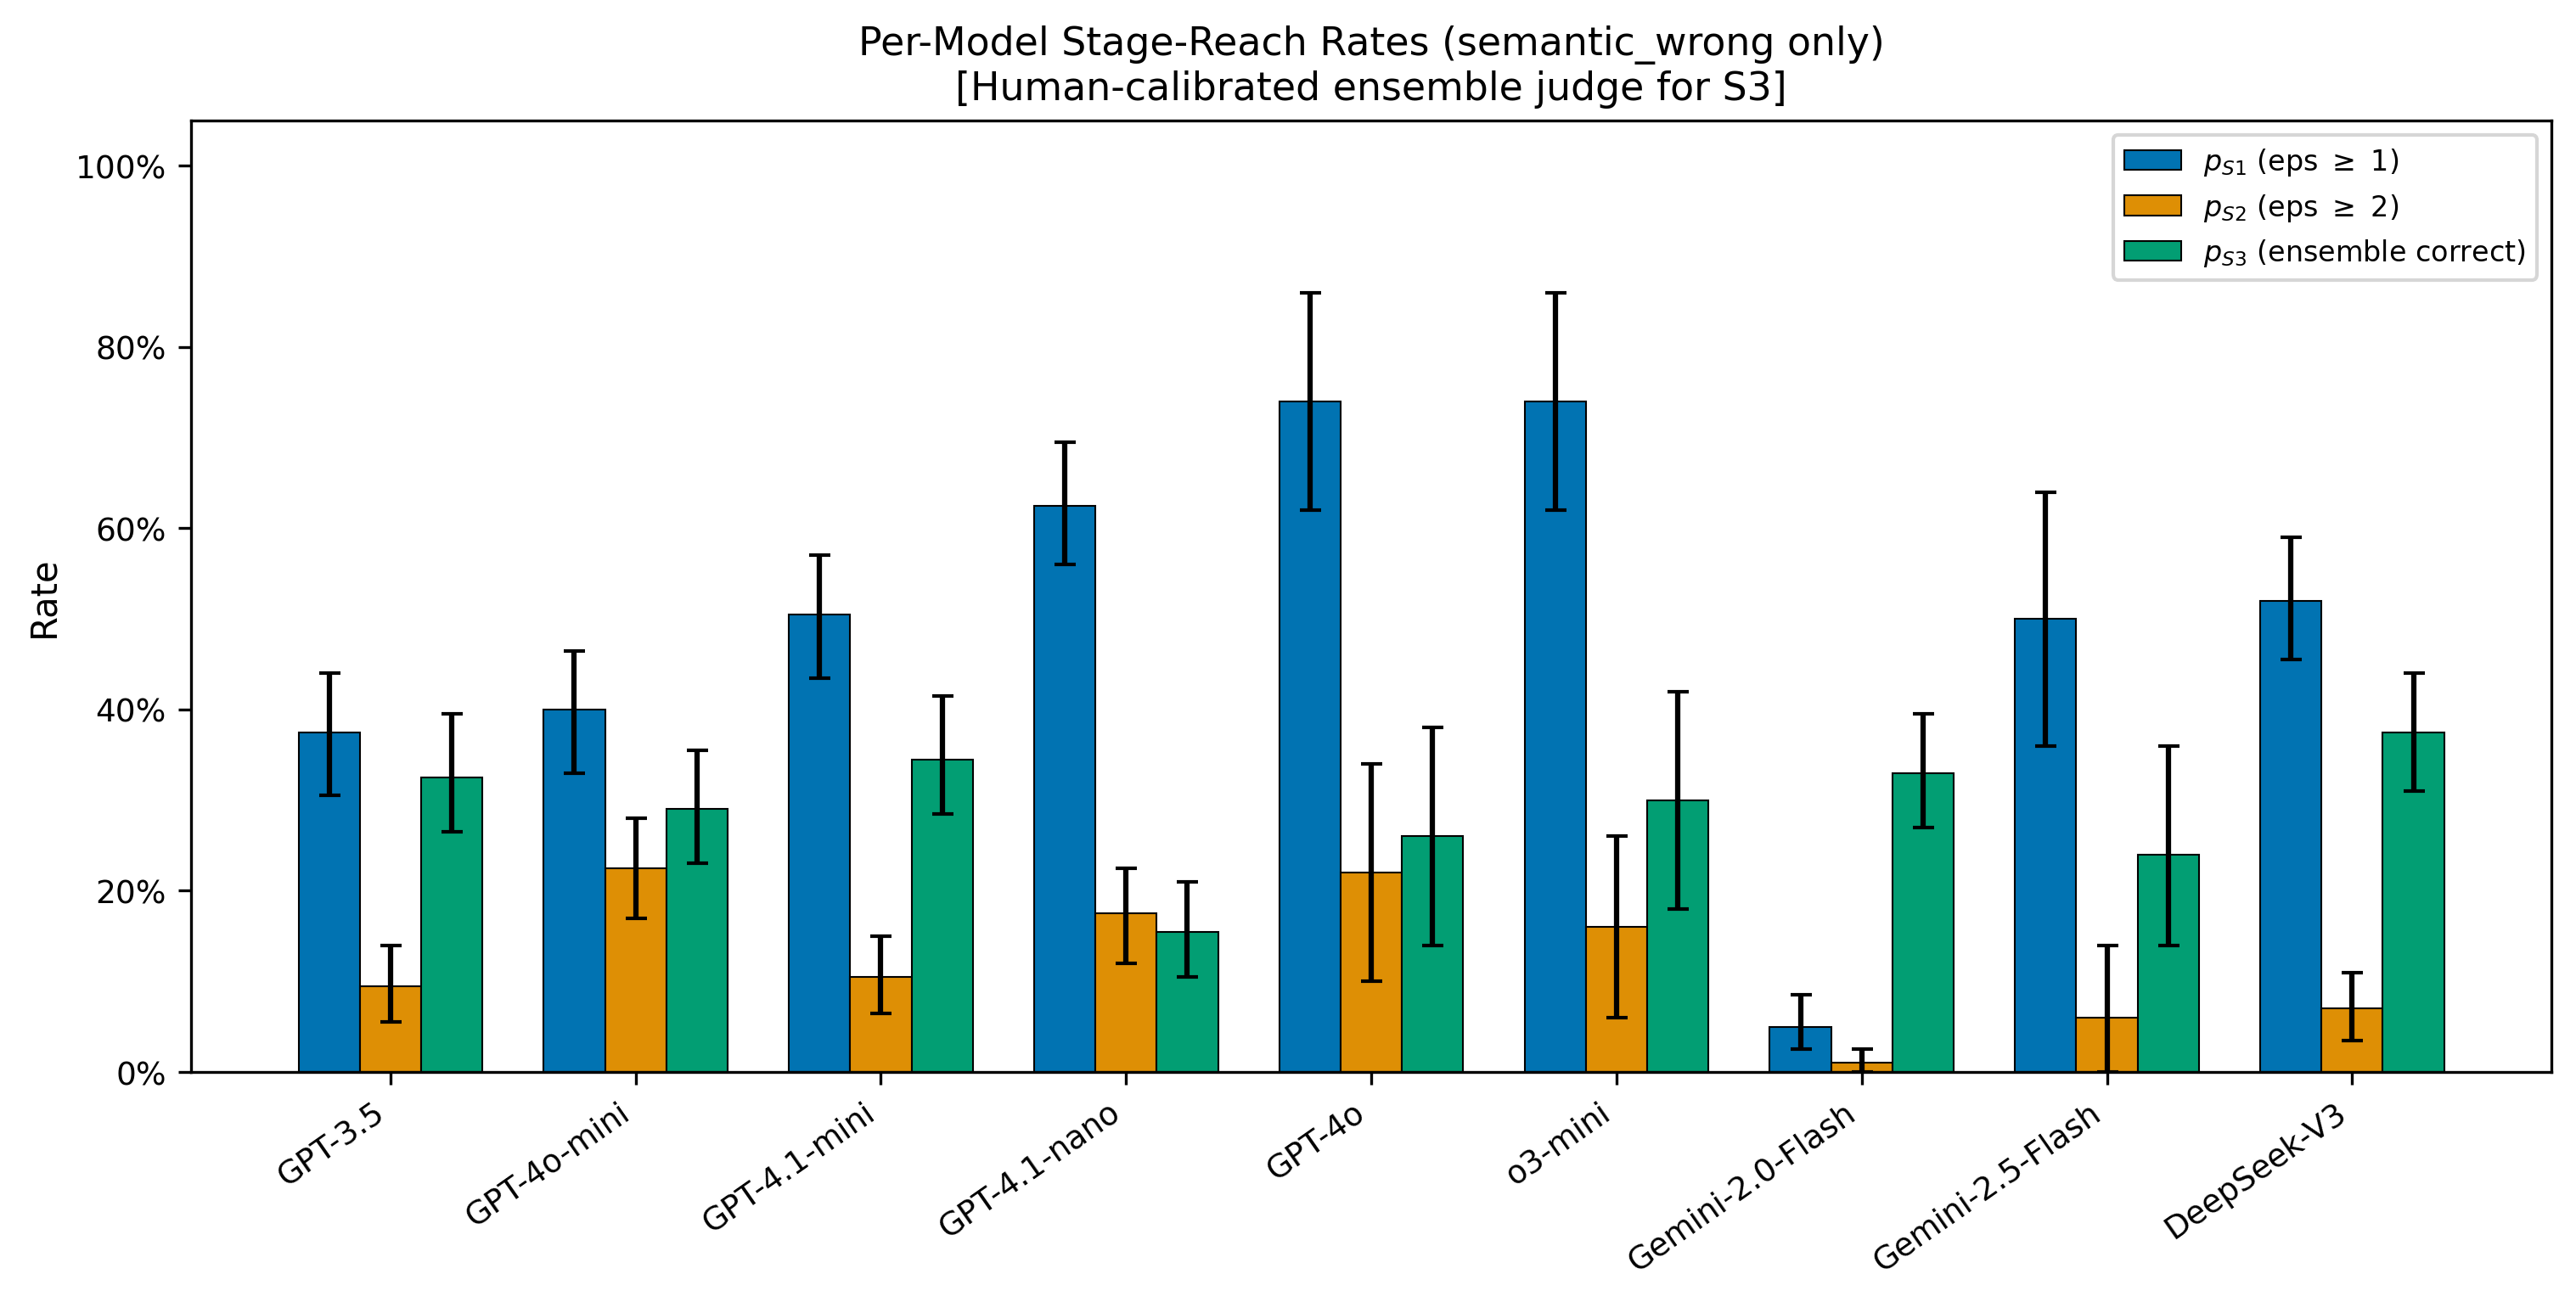
\includegraphics[width=\textwidth]{figures/fig_stage_reach.png}
  \caption{Per-model stage-reach rates under P2 semantic-wrong injection
    (ensemble-judged, $n{=}1{,}350$). $S_1$: injection applied;
    $S_2$: visible execution effect; $S_3$: wrong final answer.
    Stage indicators are computed independently.}
  \label{fig:stages}
\end{figure}

\subsection{Rejection and recovery are independent capabilities}
\label{sec:rejrec}

Table~\ref{tab:rejection_recovery} and Figure~\ref{fig:rejrec} present the
rejection--recovery decomposition across nine models.

% Source: data/results/p2_all_rejudged.csv
\begin{table}[t]
\centering
\caption{Rejection rate ($1 - P(S_1)$) versus recovery rate ($1 - r_{23}$) per model. Spearman $\rho = 0.126$, $p = 0.747$ ($n = 9$ models), indicating no significant monotonic relationship between a model's propensity to reject injected errors and its ability to recover from propagated ones.}
\label{tab:rejection_recovery}
\begin{tabular}{l r r r}
\toprule
Model & Rejection\% & Recovery\% & $n_{S_2}$ \\
\midrule
DeepSeek-V3 & 48.0 & 57.1 & 14 \\
GPT-3.5-Turbo & 62.5 & 26.3 & 19 \\
GPT-4.1-mini & 49.5 & 33.3 & 21 \\
GPT-4.1-nano & 37.5 & 2.9 & 35 \\
GPT-4o & 26.0 & 18.2 & 11 \\
GPT-4o-mini & 60.0 & 15.6 & 45 \\
Gemini-2.0-Flash & 95.0 & 50.0 & 2 \\
Gemini-2.5-Flash & 50.0 & 33.3 & 3 \\
o3-mini & 26.0 & 37.5 & 8 \\
\bottomrule
\end{tabular}
\end{table}

\begin{figure}[t]
  \centering
  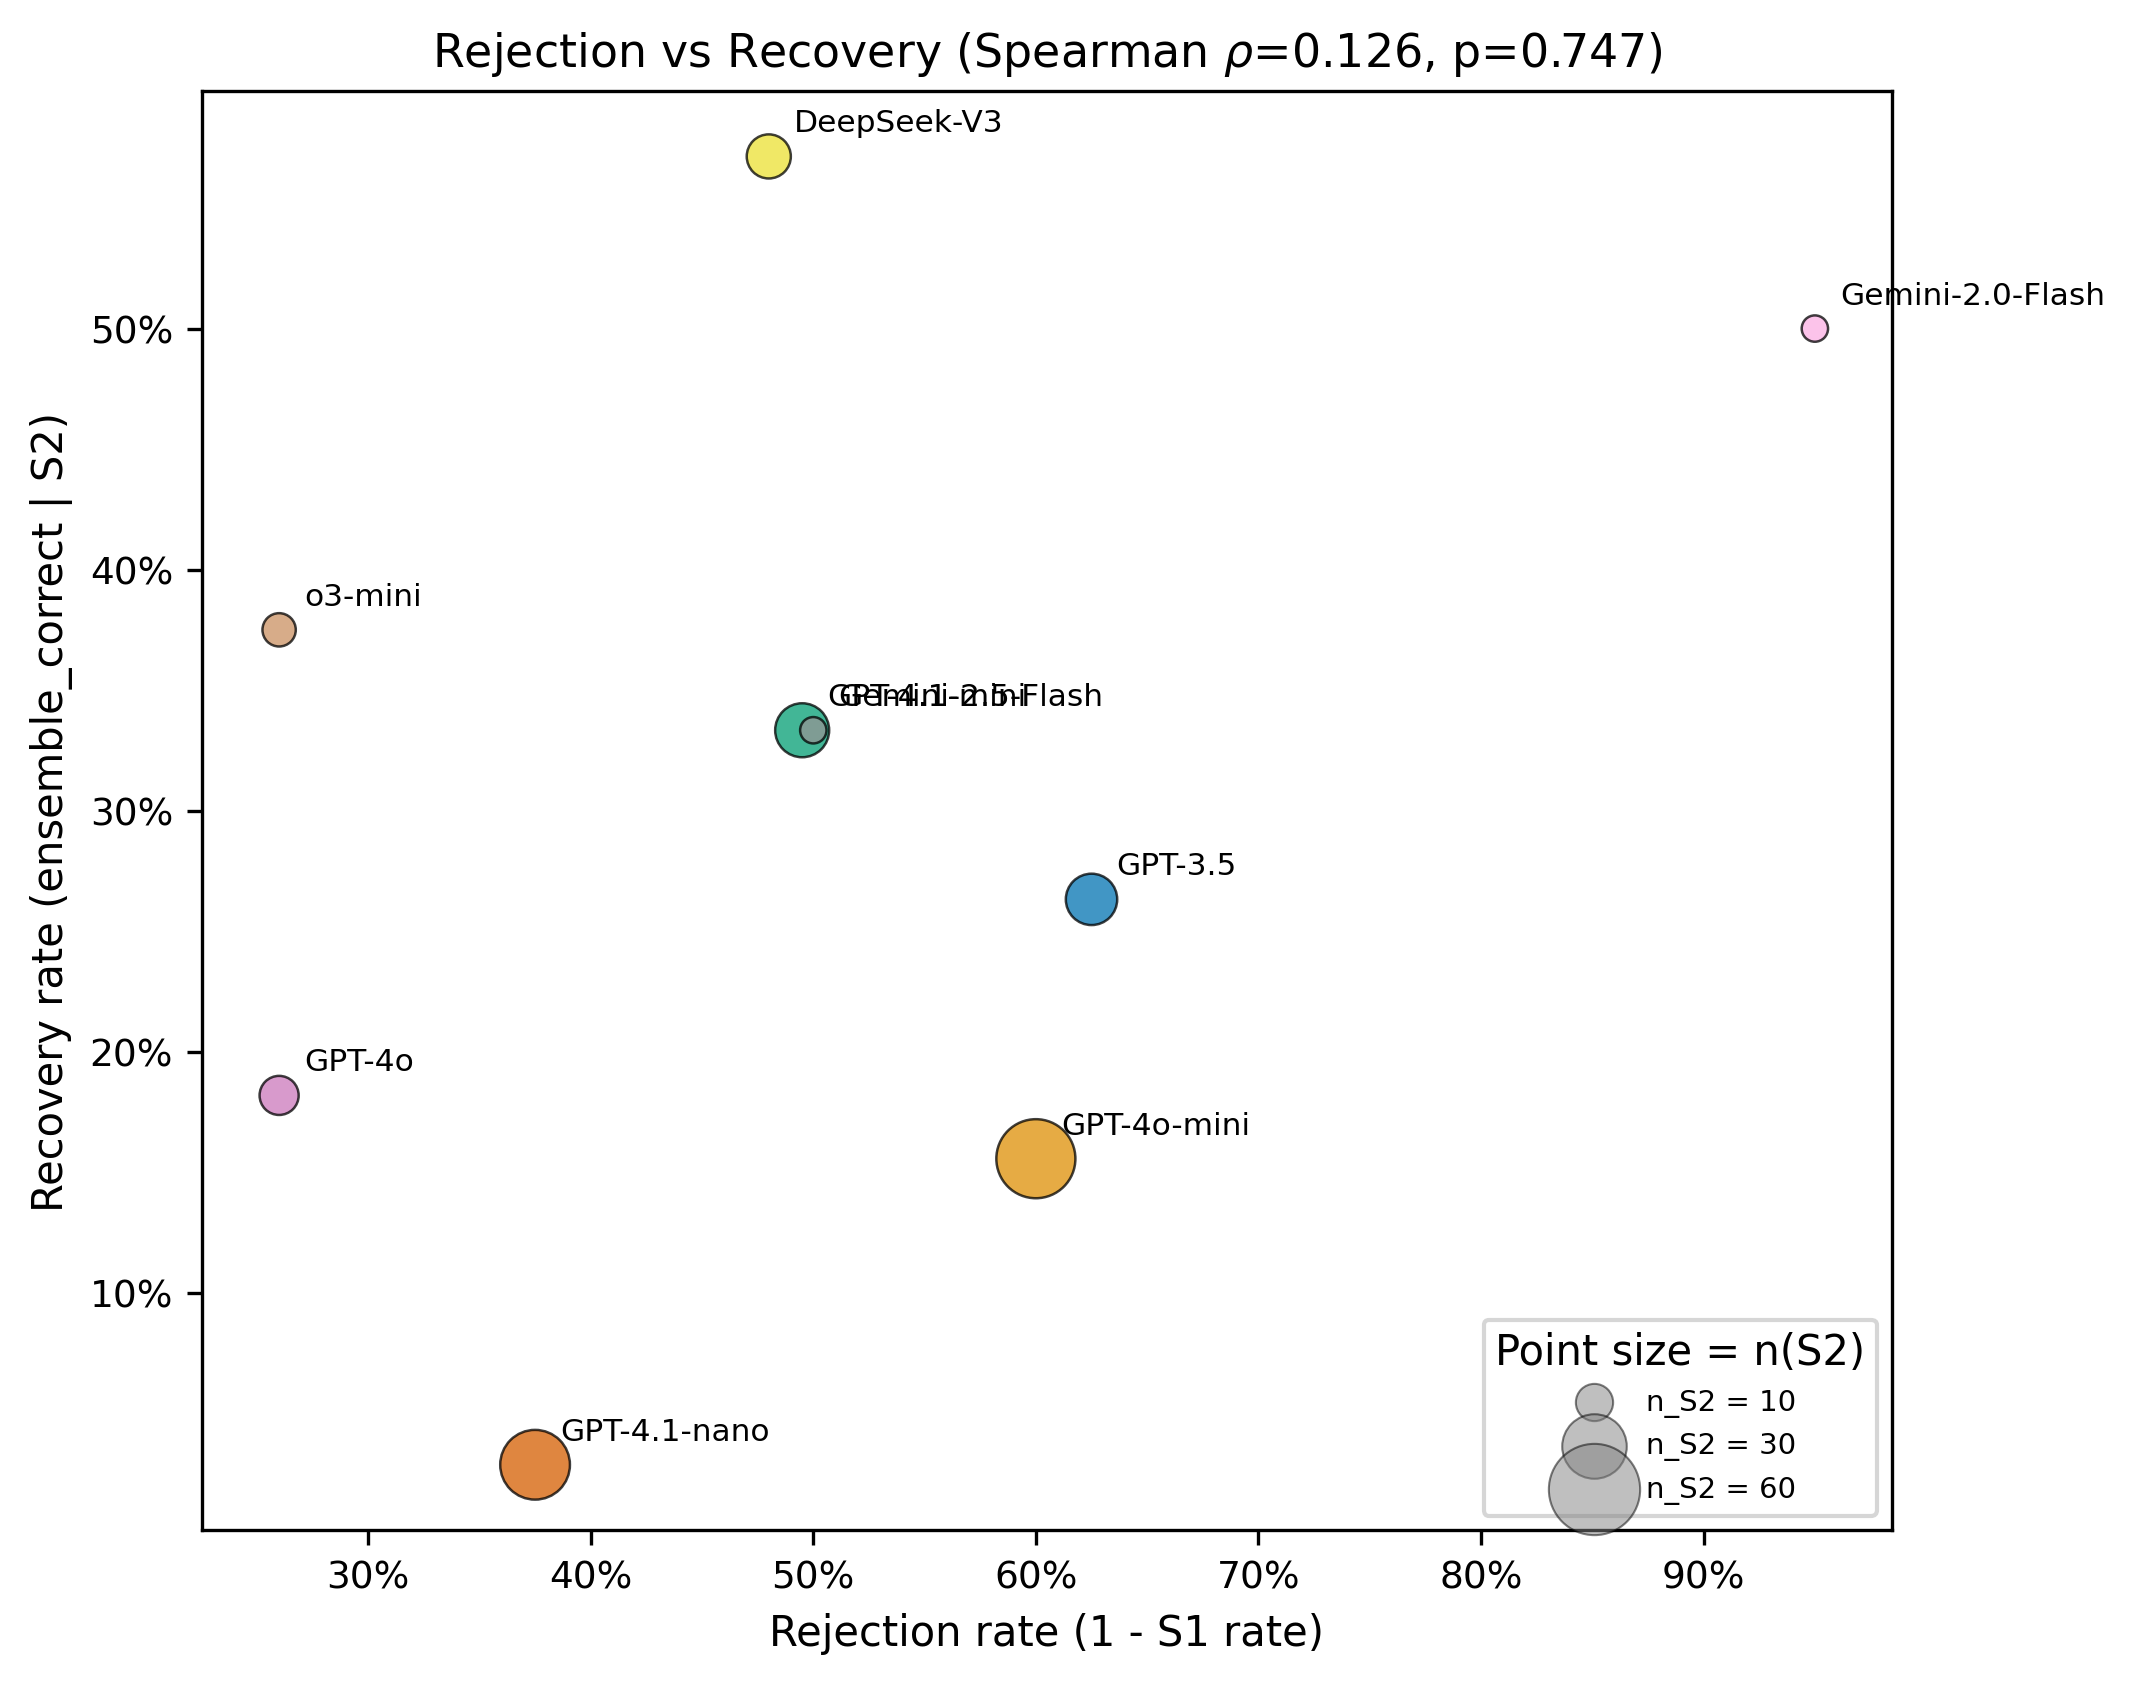
\includegraphics[width=0.7\textwidth]{figures/fig_rejection_vs_recovery.png}
  \caption{Rejection rate ($1{-}p_{S_1}$) vs.\ recovery rate
    ($1{-}r_{2,3}$) for nine models. Point size proportional to
    $n_{S_2}$. Spearman $\rho{=}0.126$, $p{=}0.747$: axes are
    statistically independent.}
  \label{fig:rejrec}
\end{figure}

Spearman rank correlation between rejection rate and recovery rate is
$\rho{=}0.126$ ($p{=}0.747$), indicating no significant relationship.
Models occupy a two-dimensional plane rather than a single quality axis:
\begin{itemize}
  \item \textbf{Gemini-2.0-Flash}: highest rejection (95\%) and moderate
    recovery (50\%)---its aggressive parameter filtering prevents most
    injections from executing.
  \item \textbf{GPT-4.1-nano}: moderate rejection (37.5\%) but near-zero
    recovery (2.9\%)---once an injection passes the schema gate, the
    model almost never recovers.
  \item \textbf{GPT-4o-mini}: moderate rejection (60\%) but low recovery
    (15.6\%)---once an injection passes, the model rarely recovers.
\end{itemize}

This decomposition has a practical implication: improving a model's
schema validation (rejection) will not improve its ability to reason
through corrupted observations (recovery), and vice versa.
Mitigation strategies should target both axes independently.

\subsection{Runtime interceptor}
\label{sec:interceptor}

Table~\ref{tab:interceptor} reports the concurrent-control interceptor
experiment.

% Source: data/results/interceptor_control_600.csv, interceptor_heldout_600.csv
% Saved = control hallucinated AND interceptor did not hallucinate (correct or abstained)
% Broken = control did not hallucinate AND interceptor hallucinated
\begin{table}[t]
\centering
\caption{Interceptor concurrent-control experiment ($n{=}600$ per model per arm). ``Saved'': control hallucinated but interceptor did not. ``Broken'': control was non-hallucinating but interceptor hallucinated. 95\% CIs on $\Delta$ via 1{,}000-iteration bootstrap.}
\label{tab:interceptor}
\small
\begin{tabular}{l r r r l r r r}
\toprule
Model & Ctrl hall.\% & Int.\ hall.\% & $\Delta$ pp & 95\% CI & Abstain\% & Saved & Broken \\
\midrule
GPT-4o-mini & 55.8 & 32.8 & $-23.0$ & [$-28.5$, $-17.3$] & 33.5 & 163 & 25 \\
Gemini-2.0-Flash & 44.5 & 43.2 & $-1.3$ & [$-7.3$, $+4.2$] & 2.8 & 24 & 16 \\
\bottomrule
\end{tabular}
\end{table}


\paragraph{GPT-4o-mini.}
The interceptor reduces hallucination from 55.8\% (control) to 32.8\%
(interceptor), a $-23.0$ percentage-point reduction.
The interceptor saved 163 traces that would have been wrong and broke
25 that would have been correct.
Analysis of the 25 broken traces revealed zero interceptor abstentions
and no domain clustering---the failures are attributable to LLM
run-to-run variance, not systematic false positives from the
interceptor.

\paragraph{Gemini-2.0-Flash.}
The interceptor has no significant effect: 44.5\% (control) vs.\
43.2\% (interceptor), $\Delta{=}{-}1.3$~pp, well within noise.
The interceptor's abstention rate is only 2.8\%.
This null result is consistent with the rejection--recovery analysis:
Gemini rejects 95\% of injections at the parameter stage, leaving the
interceptor with almost no target failure mode to catch.

\paragraph{Honest limitation.}
The $-23.0$~pp delta is measured under heuristic judging applied
identically to both arms.
The delta is robust to shared judging bias (any systematic over- or
under-counting affects both arms equally).
However, the absolute hallucination rates in each arm (55.8\% and
32.8\%) have not been validated by human labeling.
Validating these absolute rates would require additional human
annotation of the interceptor runs, which we leave to future work.

\begin{figure}[t]
  \centering
  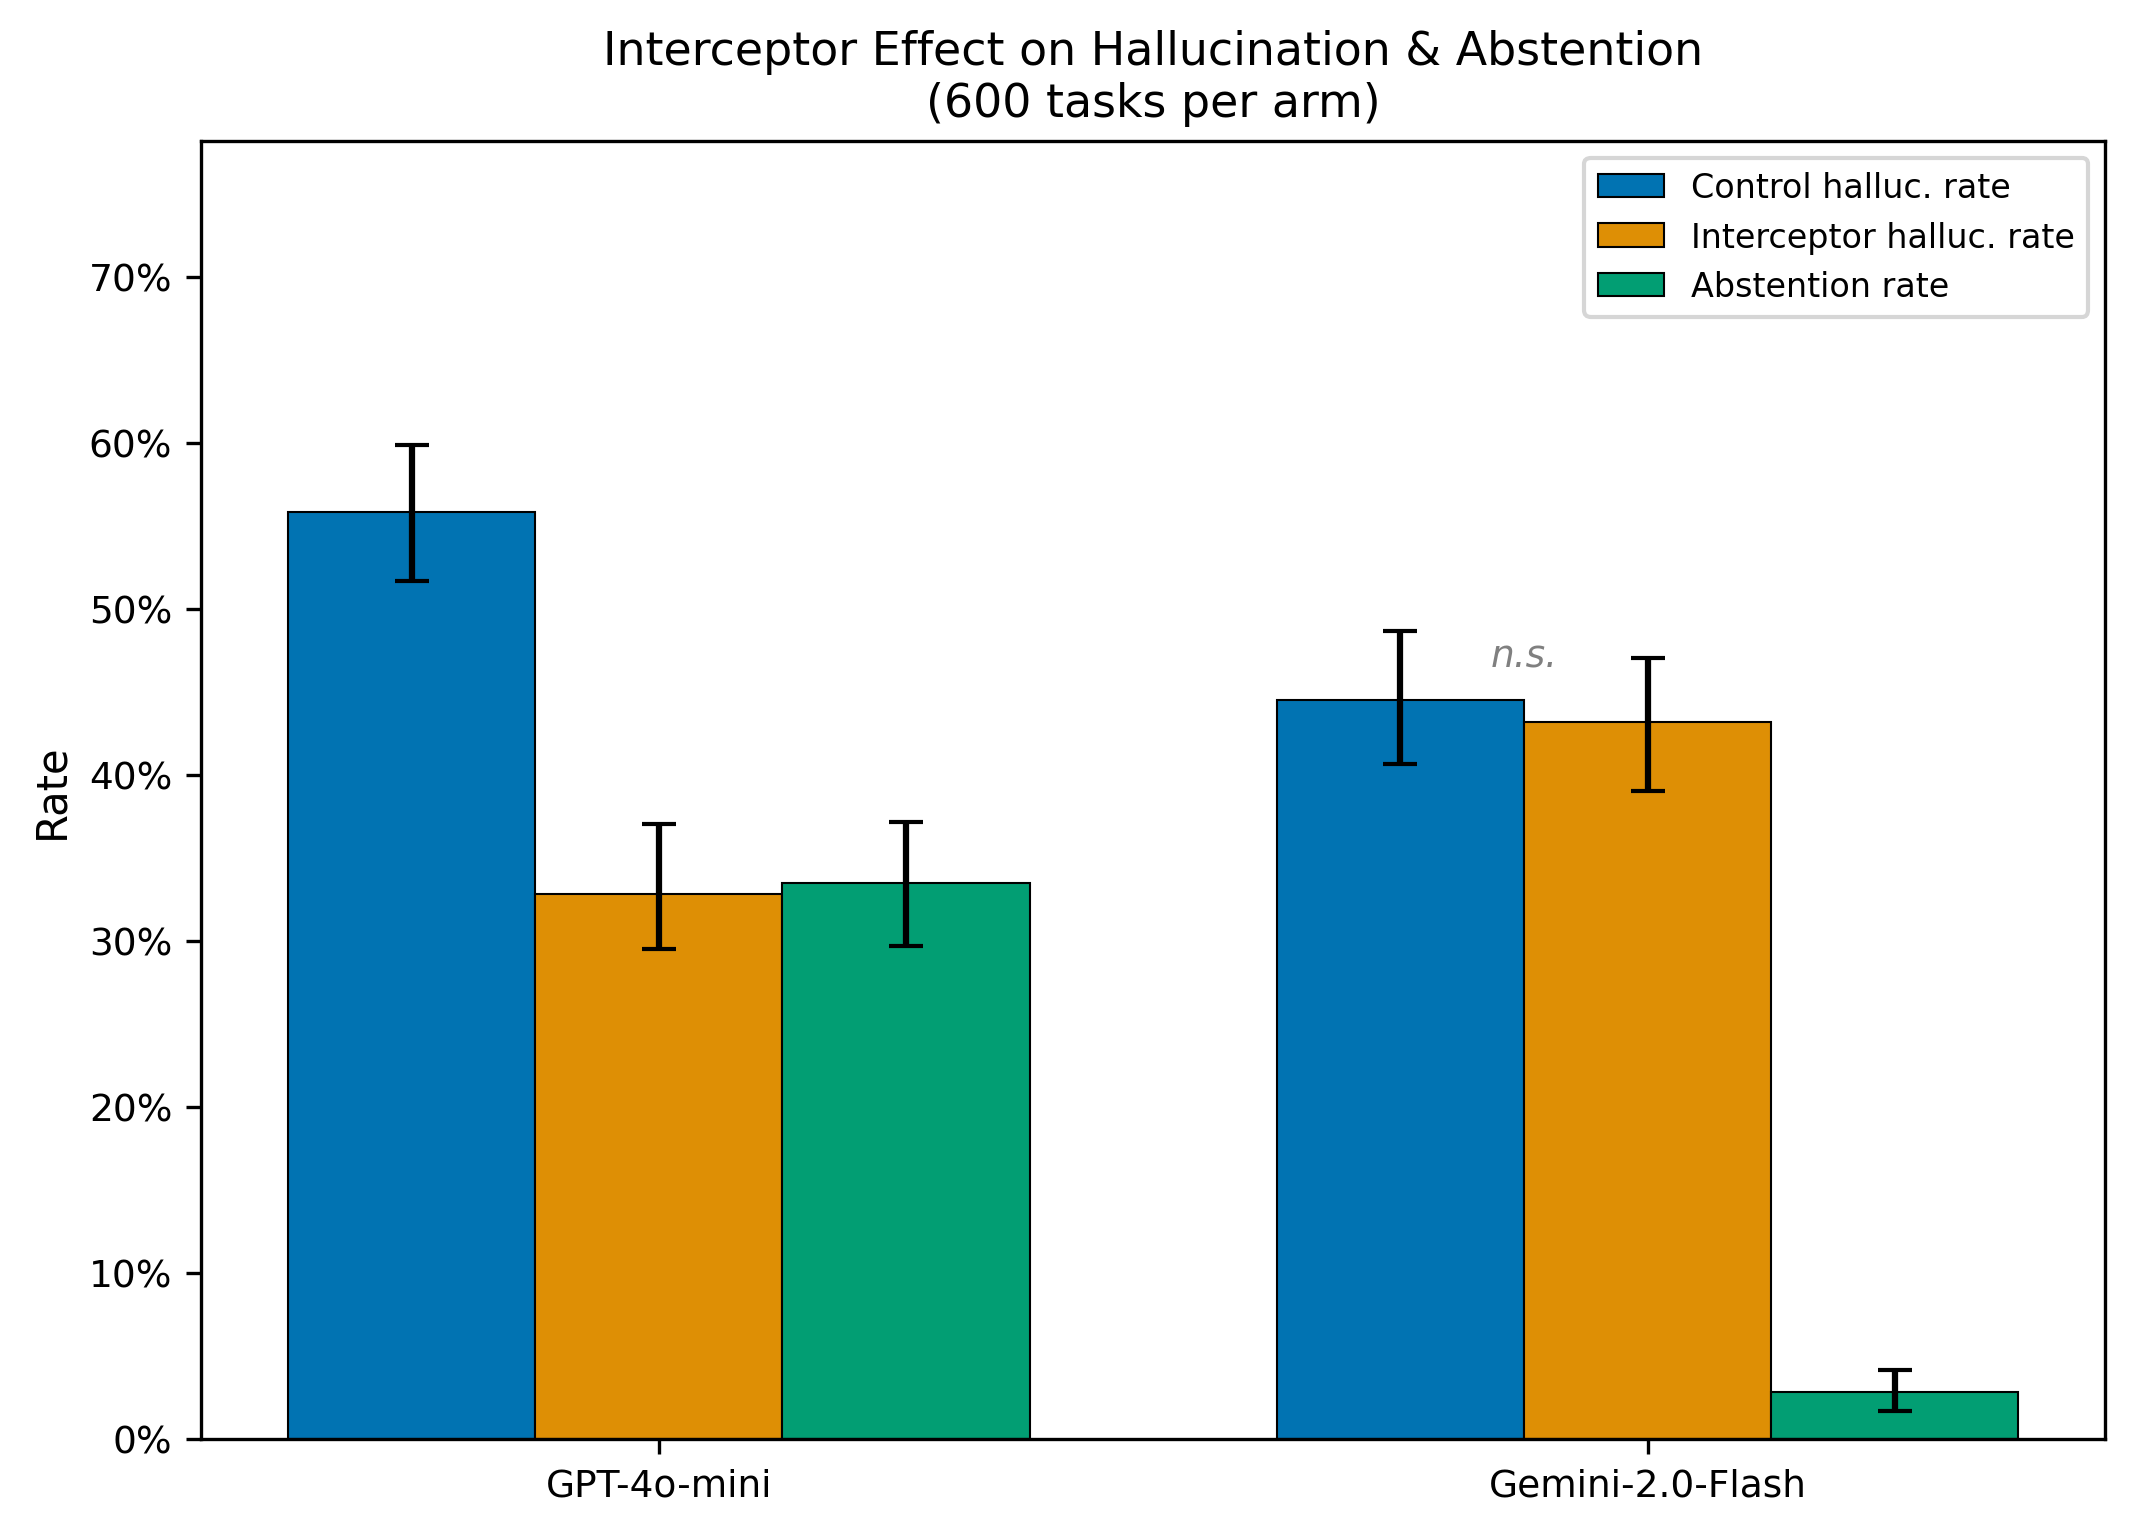
\includegraphics[width=0.7\textwidth]{figures/fig_interceptor_effect.png}
  \caption{Interceptor effect under concurrent $n{=}600$ control.
    GPT-4o-mini shows a significant 23~pp reduction; Gemini-2.0-Flash
    shows no significant effect. Error bars: 95\% bootstrap CIs.}
  \label{fig:interceptor}
\end{figure}

\subsection{Cross-domain replication on held-out retail}
\label{sec:retail}

To test generalization, we ran baseline and P2 experiments on 300
held-out retail tasks for three models.
Baseline correctness is lower on retail (harder three-tool chains),
but the model rank ordering is preserved on both correctness and mean
EPS, consistent with the original-domain results.

\begin{figure}[t]
  \centering
  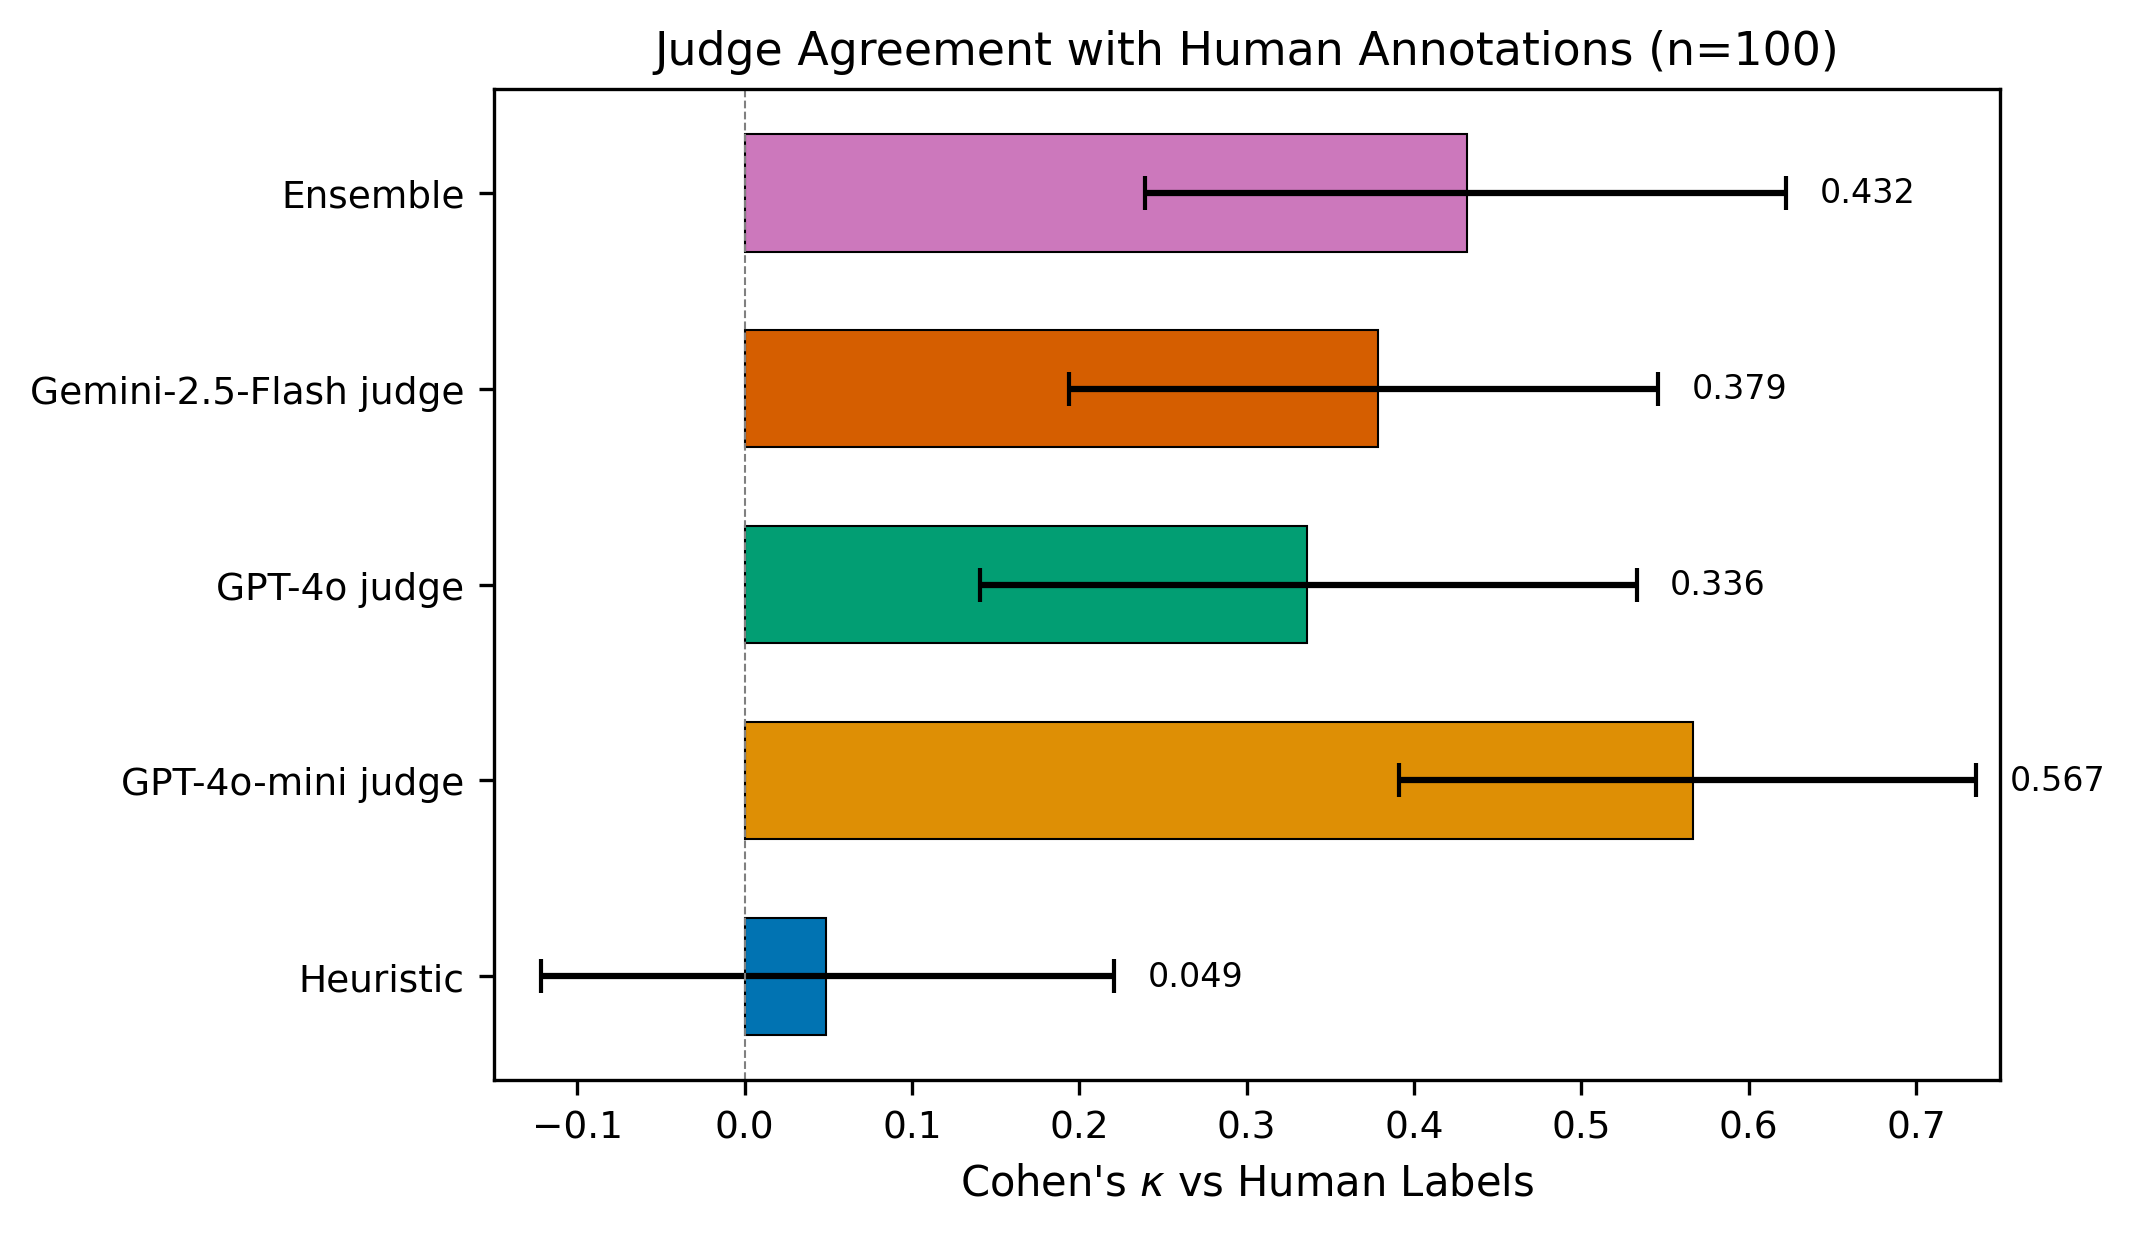
\includegraphics[width=0.65\textwidth]{figures/fig_judge_agreement.png}
  \caption{Cohen's $\kappa$ vs.\ 100 human labels for each judge method.
    The heuristic is at chance level ($\kappa{=}0.049$); the ensemble
    reaches moderate agreement ($\kappa{=}0.432$). Error bars: 95\%
    bootstrap CIs.}
  \label{fig:judge}
\end{figure}


% ============================================================================
\section{Discussion and Implications}
\label{sec:discussion}

\subsection{Theoretical implications}

\paragraph{Rejection and recovery as orthogonal axes.}
The finding that rejection rate and recovery rate are statistically
independent (Spearman $\rho{=}0.126$, $p{=}0.747$) suggests that agent
robustness to tool-use errors is at least two-dimensional.
A model's ability to reject bad parameters at the schema gate is
architecturally distinct from its ability to reason through corrupted
observations.
This has implications for how we model agent reliability: a single
``robustness score'' is insufficient; instead, practitioners should
evaluate both the input-filtering and the output-reasoning capabilities
of an agent independently.

\paragraph{Why heuristic evaluation misranks models.}
The heuristic over-counted correctness by 34 percentage points on P2
traces, enough to reverse the direction of the baseline-vs-P2
comparison.
This occurs because injected errors produce paraphrased wrong answers
that contain enough keywords to pass substring matching.
Any benchmark that uses heuristic evaluation on agent outputs with
high output variability risks similar misranking.

\subsection{Practical implications for agent designers}

\paragraph{Schema validators are high-leverage.}
Gemini-2.0-Flash's 95\% rejection rate demonstrates that strict
parameter validation can prevent most injection-type errors from
reaching the tool-execution stage.
Designers should invest in comprehensive tool schemas with explicit
type, range, and enum constraints.

\paragraph{Pre-execution semantic checks.}
The \interceptor's L1 (schema) and L2 (keyword) layers provided the
bulk of its discriminative power.
For models with moderate rejection rates (e.g., GPT-4o-mini at 60\%),
a runtime interceptor can halve the hallucination rate at minimal cost
(\$0.15 for 1{,}200 runs).

\paragraph{Interceptors are model-dependent.}
The null result on Gemini-2.0-Flash shows that interceptors are not
universally effective.
When a model already rejects most errors at the parameter stage, there
is nothing left for the interceptor to catch.
Deployment decisions should be informed by model-specific rejection
rates.

\subsection{Implications for IR and IS evaluation}

\paragraph{Substring heuristics should be deprecated.}
Our $\kappa{=}0.049$ result is the lowest heuristic-vs-human agreement
we are aware of in any agent or QA evaluation study.
The IR community has already raised concerns about automated evaluation
reliability \citep{soboroff2024dont,thomas2024searcher}.
Our result provides concrete evidence that substring heuristics are
worse than coin flips in the agent-evaluation context.

\paragraph{LLM-ensemble judges need validation.}
The ensemble's $\kappa{=}0.432$ is a significant improvement but falls
short of the substantial-agreement threshold ($\kappa{>}0.60$).
The ensemble has a measured conservative bias, underreporting
correctness by ${\sim}13$~pp relative to humans.
We recommend that any study using LLM judges report: (a)~agreement with
at least 50 human labels, (b)~the direction of bias (conservative vs.\
permissive), and (c)~calibrated estimates alongside raw judge outputs.

\paragraph{Methodology transfers to RAG and QA evaluation.}
The three-judge ensemble protocol, the human-calibration procedure, and
the independence-testing framework for evaluation axes all apply to RAG
pipeline evaluation, open-domain QA, and any setting where output format
variability makes heuristic matching unreliable.

\subsection{Differentiation from existing work}

Table~\ref{tab:diff} positions \bench{} relative to four closely related
benchmarks.

\begin{table}[h]
\centering\small
\caption{Comparison with related benchmarks.}
\label{tab:diff}
\begin{tabular}{lcccc}
\toprule
Feature & $\tau$-bench & AgentBench & AgentHallu & \bench{} \\
\midrule
Stage-level metrics & \texttimes & \texttimes & \checkmark & \checkmark \\
Controlled injection & \texttimes & \texttimes & \texttimes & \checkmark \\
Human-validated judge & \texttimes & \texttimes & \texttimes & \checkmark \\
Runtime mitigation & \texttimes & \texttimes & \texttimes & \checkmark \\
Concurrent control & \texttimes & \texttimes & \texttimes & \checkmark \\
\# Models evaluated & 6 & 25 & 14 & 9 \\
\# Traces & 1{,}280 & 7{,}000+ & 693 & 2{,}300 \\
\bottomrule
\end{tabular}
\end{table}


% ============================================================================
\section{Limitations}
\label{sec:limits}

\begin{enumerate}
  \item \textbf{Ensemble conservative bias.}
    The ensemble judge's $P(\text{human=correct} \mid
    \text{ensemble=wrong})=0.25$ means one in four ensemble ``wrong''
    verdicts is a false negative.
    All ensemble-judged rates should be interpreted as lower bounds on
    true correctness.

  \item \textbf{Human-label sample size.}
    With $n{=}100$ labels, the calibration estimates have wide confidence
    intervals.
    The human-vs-ensemble $\kappa{=}0.432$ has a 95\% CI of approximately
    $[0.28, 0.58]$ by bootstrap.
    This is moderate, not definitive, validation.
    The annotator was the first author; a second annotator independently
    labeled 7 overlapping traces with 6/7 agreement.
    Future work should use a larger non-author annotator pool to
    eliminate any potential annotator bias.

  \item \textbf{Interceptor absolute rates.}
    The interceptor delta ($-23.0$~pp) is robust to shared heuristic
    judging bias, but the absolute hallucination rates (55.8\% and
    32.8\%) are unvalidated by human annotation.
    Future work should apply human labeling to the interceptor arms.

  \item \textbf{Model selection.}
    We evaluated nine API-accessible models.
    Open-weight models (Llama, Qwen) were excluded because injection
    requires intercepting the tool-call pipeline before execution, which
    is more complex with local inference.
    Claude models were excluded to avoid potential evaluation conflicts.

  \item \textbf{Simulated tools.}
    All tool calls execute against deterministic simulators, not live
    APIs.
    Live API variability (rate limits, format changes, partial failures)
    may introduce additional propagation pathways not captured here.

  \item \textbf{Single-parameter injection.}
    We inject one parameter per trace.
    Multi-parameter and multi-turn injection (P3 memory accumulation,
    P4 cross-agent propagation) are deferred to future work.

  \item \textbf{Scope.}
    This paper covers only the P2 parameter-injection protocol.
    P3 (memory-accumulation propagation across turns) and P4
    (cross-agent pipeline propagation) share the EPS machinery but
    require different task formats and are deferred.

  \item \textbf{Small per-model $n_{S_2}$ samples.}
    The stage-2 subset sizes $n_{S_2}$ range from 2 (Gemini-2.0-Flash)
    to 45 (GPT-4o-mini).
    Per-model $r_{2,3}$ estimates for models with $n_{S_2} < 10$ have
    wide confidence intervals (e.g., CI $[0, 1]$ for $n_{S_2}{=}2$)
    and should be interpreted as directional only.
    The marginal injection-to-error rate $\Pr[S_3 \mid S_1]$, computed
    on the larger $S_1{=}1$ subset, provides a more stable summary.

  \item \textbf{Power of the independence test.}
    The Spearman correlation between rejection and recovery rates is
    computed across $n{=}9$ models.
    With this sample size, only strong monotonic relationships
    ($|\rho| > 0.7$) would be detectable at conventional significance
    levels.
    Our finding ($\rho{=}0.126$, $p{=}0.747$) is consistent with
    genuine independence but also with a moderate underlying relationship
    the test cannot detect.
    We report it as \emph{no evidence of correlation} rather than
    \emph{proof of independence}.
\end{enumerate}


% ============================================================================
\section{Conclusion}
\label{sec:conclusion}

We introduced \bench{}, a benchmark for evaluating tool-using LLM agents
with validated judging, stage-level propagation measurement, and a
runtime mitigation evaluated under concurrent control.

\paragraph{RO1 (Judge reliability).}
Substring-based evaluation of agent outputs agrees with human annotation
at $\kappa{=}0.049$ (chance-level).
A three-LLM ensemble reaches $\kappa{=}0.432$ (moderate) with a
conservative bias.
We recommend that all agent benchmarks validate their evaluation
methodology against human labels before reporting comparative claims.

\paragraph{RO2 (Propagation).}
Under validated evaluation, a parameter-level injection propagates to a
wrong final answer with human-calibrated probability ${\approx}\,0.62$
(range 0.46--0.73 across models).
Rejection rate and recovery rate are independent capabilities
(Spearman $\rho{=}0.126$, $p{=}0.747$), indicating that model
robustness to tool-use errors is at least two-dimensional.

\paragraph{RO3 (Mitigation).}
A lightweight runtime interceptor reduces GPT-4o-mini hallucination by
23 percentage points under a concurrent $n{=}600$ control.
The effect is model-dependent: Gemini-2.0-Flash shows no effect because
its aggressive parameter rejection eliminates the target failure mode.

All code, data, 2{,}300 traces, and 100 human labels are released at
\url{https://github.com/bhaskargurram-ai/agenthallu-bench} to support
reproducible agent evaluation research.


% ============================================================================
\bibliographystyle{plainnat}
\bibliography{refs}

\end{document}
